% Chapter 2

\chapter{Films polim\'ericos} % Main chapter title

\label{Chapter-film} % For referencing the chapter elsewhere, use \ref{Chapter1}

\section{Introducci\'on/Motivaci\'on}

En esta secci\'on nos valdremos de una  red polim\'erica que da estructura de un  film polim\'erico entrecruzado, un hidrogel. 
Como se mencion\'o antes los films son materiales ampliamente investigados para aplicaciones biom\'edicas. \addcite 
La respuesta a est\'imulo y su capacidad para adsorber grandes cantidades de solventes los hace muy atractivos al momento de adsorber drogas/prote\'inas de interes terapeutico. \addcite
Este sistema adem\'as de poder explicar la fisicoqu\'imica que lo envuelve, y poder responder respuestas a comportamientos observados experimentalmente \addcite fue una introducci\'on  en la teor\'ia molecular.
La derivaci\'on de cada componente energ\'etico, la confecci\'on de los modelos moleculares as\'i como tambi\'en la escritura de los c\'odigos forman parte de este primer cap\'itulo. Son el puntap\'ie para poder aplicarlo a los sistemas de micro y nano geles.
La importancia de este primer cap\'itulo tambi\'en radica en el entendimiento de algunos conceptos que ser\'an aplicados a lo largo de esta tesis. La respuesta a pH y sus cambios en ambientes confinados, el ambiente de un hidrogel, y la regulaci\'on de carga de las diferentes especies presentes en el sistema son detalladas a continuaci\'on.


\begin{figure}
	\centering
	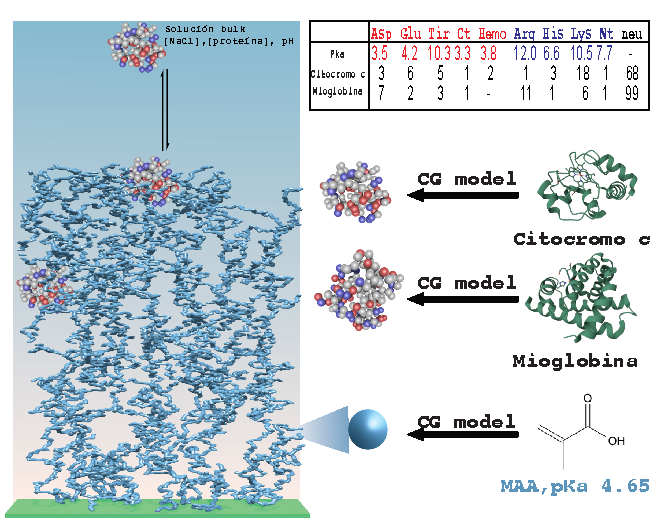
\includegraphics[width=0.9\textwidth]{Figures/graph-film/film_model.pdf}
	\caption{Esquema de simulaci\'on de un film polim\'erico compuesto por MAA. Se muestra adem\'as las prote\'inas usadas y el modelo de grano grueso. En la tabla se ven los segmentos que componen al modelo y la informaci\'on de los pKa asociadas a cada una de ellas.}
	\label{fig:film:model_film}
\end{figure}



\section{Te\'oria Molecular } \label{sec:film-teoria}

El m\'etodo propuesto consiste en minimizar una energ\'ia libre generalizada que incluye toda la termodinamica relevante que engloba los procesos del sistema polim\'erico con una soluci\'on.
Para tal fin se usamos  una descripci\'on molecular de grano grueso de las diferentes especies qu\'imicas que componen el sistema.
Dicha descripci\'on incluye forma, tama\~no, distribuci\'on de carga (si los hubiese) y estado de protonaci\'on de cada componente molecular en los casos que corresponda.
En esta primera instancia describiremos la fisicoqu\'imica de un film  se encuentra en  equilibrio con una soluci\'on acuosa, la tiene una composici\'on  definida externamente (ba\~no de la soluci\'on).
Es decir, el pH, la concentración de sal y la concentraci\'on de adsorbatos son variables independientes.


Nuestro film que posee distintos tipos de segmentos: una unidad sensible al pH, en particular consideraremos un film polim\'erico compuesto por unidades \'acidad de \'acido metacr\'ilico ($MAA$).
Este film est\'a  se encuentra en equilibrio con una soluci\'on con una temperatura, pH y concentraci\'on de sal definidas. Adem\'as vamos a considerar que en dicha soluci\'on hay un adsorbato, en este cap\'itulo usaremos una prote\'ina, la cual puede ser cictocromo c o mioglobina. 
Considerando los aspectos anteriores es posible definir una energ\'ia libre:

\begin{align}
 	F = -TS_{mez} -TS_{conf,net} + F_{qca,net} + F_{qca,pro} + U_{elec} + U_{ste} + U_{VDW}
 	\label{eq:film:libre-film}
\end{align}
 
\noindent En donde $S_{mez}$ es la entrop\'ia de traslaci\'on ( y de mezcla) de las especies libres en la soluci\'on: mol\'eculas de agua (H$_2$O), y sus respectivos iones:  hidronio (H$_3$O$^+$), e hidr\'oxido (OH$^- $), cationes y aniones de sal y nuestra prote\'ina modelo.
Aqu\'i, consideramos una sal monovalente, NaCl, la cual est\'a completamente disociada en sus  iones cloruro (Cl$^-$) y sodio ($Na^+$). 

$S_{conf,nw}$ representa la entrop\'ia conformacional que resulta de la flexibilidad de la red de polim\'erica, la cual viene dada por todas las conformaciones diferentes que puede asumir la misma.

$F_{qca,net}$, es la energ\'ia qu\'imica libre que describe el equilibrio entre las especies protonadas y desprotonadas de unidades funcionales (\'acidas/b\'asicas), para nuestro film solo se consideran unidades \'acidas.

De manera similar, $F_{qca,net}$ describe la protonaci\'on de residuos titulables de la prote\'ina.

$U_{elec}$ y $U_{ste}$ representan, respectivamente, las interacciones electrost\'aticas y las repulsiones est\'ericas.
Las interacciones de Van der Waals son representadas en $U_{VdW}$.


Las expresiones explicitas de la ecuaci\'on \ref{eq:film:libre-film} las describimos acontinuaci\'on.

Como primer termino tenemos la entrop\'ia de mezcla de  las especies mobiles, entre ellas consideramos a nuestra prote\'ina modelo:

\begin{align}
	\begin{aligned}
		-\frac{S_{mez}}{k_B}= &A\sum_{\gamma}\int_0^\infty{dz\rho_\gamma(z)\left(\ln \left(\rho_\gamma (z)v_w\right) -1 + \beta\mu^0_\gamma\right)} \\
		&+ A\sum_{\theta}\int_0^\infty{dz\rho_{pro}(\theta,z)\left(\ln \left(\rho_{pro}(\theta,z)\right) -1 + \beta\mu^0_{pro} \right)}
	\end{aligned}
\end{align}

\noindent en donde $\frac{1}{k_B T}$, y $k_B$ es la constante de Boltzmann, $T$ es la temperatura absoluta del sistema. La variable $z$ es la coordenada que mide la distancia a la superficie de soporte de nuestro film, el \'ara total de esta superficies es $A$. $\rho_\gamma(z)$ y $\mu_\gamma$ es densidad local, a un $z$ dado, y potencial qu\'imico estadar de la especie $\gamma$ respectivamente.
El subinidice $\gamma$ toma en cuenta la mol\'ecula de agua y sus respectivos ione (hidronio e hidr\'oxido), adem'as de los iones provenientes de la sal ($Na^+$ y $Cl^-$). 


El segundo t\'ermino de esta ecuaci\'on corresponde a la entrop\'ia de mezcla de la prote\'ina. $\rho_{pro}(\theta,z)$ es la densidad local de la prote\'ina en la conformaci\'on $\theta$. Es decir $\theta$ recorre sobre las configuraciones de la misma.
Esta conformaciones incluyen rotaciones espaciales de la prote\'ina.
De este modo la densidad local media de la prote\'ia puede expresarse como:


\begin{align}
	\left<\rho_{pro}(z)\right> = \sum_\theta{\rho_{pro}(\theta,z)}
\end{align}


La entrop\'ia conformational que resutla de la flexibilidad de la red polim\'erica de nuestro film se representa en $S_{conf, nw}$, esta tiene en cuenta todas las configuraciones de un set $\{\alpha\}$.

\begin{equation}
	\frac{S_{conf,net}}{k_B} = - \sum_{\alpha}{P(\alpha)\ln P(\alpha)}
\end{equation}

\noindent en donce $P(\alpha)$ denota la probabilidad de que el film se encuentre en la configuraci\'on $\alpha$.

El siguiente t\'ermino de eq \ref{eq:film:libre-film} describe  la energ\'ia libre dada por  el equilibrio \'acido-base de los segmentos de MAA que componen nuestra red. 

\begin{align}
	\begin{aligned}
		\beta F_{qca,net} &= A\int_0^\infty dz \left<\rho_{MAA}(z)\right> \left[f(z)(\ln f(z)+ \beta\mu^0_{MAA^-})\right.\\
		&\left.+(1-f(z))(\ln (1-f(z))+\beta\mu^0_{MAAH})\right]    
	\end{aligned}
\end{align} 

\noindent en donde $f(z)$ es el grado de carga de los segmentos de MAA entre las capaz $z$ y $z + dz$. 
$\mu^0_{MAA^-}$ y $\mu^0_{MAAH}$ son los potenciales qu\'imico estandar  de las especies protonadas y desprotonadas respectivamente.
Adem\'as se define:

\begin{align}
	\left< \rho_i(z)\right> = \sum_\alpha{P(\alpha)\rho_i(\alpha,z)}
\end{align}
\noindent en el cual $\rho_i(\alpha,z)$  es el ensamble de densidad  promedio local del film. El cual es una variable de entrada que cuantifica la desnidad de segmentos del film que  ocupan una capa $z$ cuando la red se encuentra en la conformaci\'on $\alpha$.


%%%%%%%%%%%%%%%%%%%
El equilibrio qu\'imico de las unidades titulables de la prote\'ina es considerada en el siguiente t\'ermino de la energ\'ia libre:

\begin{align}
	\begin{aligned}
		\beta F_{qca,pro} = A\int_0^\infty dz& \sum_\tau \left<\rho_{pro,\tau}(z)\right> \left[g_\tau(z)(\ln g_\tau(z)+ \beta\mu^0_{\tau p})\right.\\
		&\qquad\left.+(1-g_\tau(z))(\ln (1-g_\tau(z))+\beta\mu^0_{\tau d})\right]   
	\end{aligned}
\end{align} 

\noindent en donde $\left<\rho_{pro,\tau}(z)\right>$ representa la densidad local promedio del segmento protonable $\tau$ de la prote\'ina.

Que se define como:
\begin{align}
	\left<\rho_{pro,\tau}(z)\right> = A\sum_\theta \int dz^\prime  \rho_{pro}(\theta,z^\prime)n_\tau(\theta,z^\prime, z)
	\label{eq:film:segments_pro_si}
\end{align}
\noindent en donde $n_\tau(\theta,r^\prime, r)$ es un par\'ametro de entrada que nos da el n\'umero de segmentos $\tau$ entre las capas $z$ and $z+ dz$ cuando el centro de masa de la prote\'ina se encuentra en el a configuraci\'on $\theta$ y en la posici\'on $z^\prime$.

Las unidades titulables pueden estar en esta protonado $\tau, p$ o desprotonado $\tau, d$, los cuales poseen su potenciales qu\'imicos est\'andar $\mu^0_{\tau,p}$ y $\mu^0_{\tau,d}$ respectivamente. 
Adm\'as definimos el grado de asociaci\'on $g_\tau$ para segmento $\tau$ como:


\begin{enumerate}
	\item para unidades \'acidas: $g_\tau(r) = 1-f_\tau(r)$ ( las unidades $\tau$ se cargan negativamente)
	\item para unidades b\'asicas: $g_\tau(r) = f_\tau(r)$ (las  unidades $\tau$ se cargan positivamente  )
\end{enumerate}
en donde  $f_\tau(r)$ es el grado de disosiac\'on de cada segmento $\tau$.
%%%%%%%%%%

La energ\'ia electr\'ostatica se define como:
\begin{align}
	\begin{aligned}
		\beta U_{elec}= A\int_0^\infty dz&\left[\left(\sum_{\gamma } {\rho_\gamma(z) q_\gamma + \sum_\tau{f_\tau(z) \left<\rho_{pro,\tau}(z)\right> q_\tau} +  f(z)\left<\rho_{MAA}(r)\right>q_{MAA}}\right)\beta\psi(z) \right. \\ &\left.-\frac{1}{2}\beta\epsilon(\nabla\psi(z))^2 \right]
	\end{aligned}
\end{align} 

\noindent en donde $\Psi(z)$ es el potencial elestr\'ostatico dependiente de la posici\'on, $\epsilon$ es la constante de permitividad del medio, $q_\gamma$ es la carga correspondiente a la especiel m\'obil $\gamma$, $q_\tau$ es la carga que adquieren los segmentos titulables de la prote\'ina. Finalmente $q_{MAA}$ es la carga que adquiere el segmento de $MAA$ al desprotonarse.


En este contexto, la densidad de carga media es:

\begin{align}
	\left<\rho_q(z)\right> = \sum_{\gamma } {\rho_\gamma(z) q_\gamma + \sum_\tau{f_\tau(z) \left<\rho_{pro,\tau}(z)\right> q_\tau} +  f(z)\dfrac{\left<\phi_{MAA}(z)\right>}{v_{MAA}}q_{MAA}}
	\label{eq:film:rho_charge}
\end{align}
%%%%%%%%%%%%%%%%

La contribuci\'on siguiente en la energ\'ia libre viene dada por la repulsi\'on esterica entre  todos los segmentos que componen  el sistema. Esta contribuci\'on se incorpora a travez del siguiente restricci\'on:  

\begin{align}
	\begin{aligned}
		1=  {\left[\sum_{\gamma}\rho_\gamma(z) v_\gamma + \sum_\lambda{\left<\rho_{pro,\lambda}(z)\right>v_\lambda} + \left<\rho_{MAA}(z)\right>v_{MAA} \right]},~ \forall z
	\end{aligned}
	\label{eq:film:constraint}
\end{align}
\noindent en donde $v_\gamma$ , $v_\lambda$ y $v_{MAA}$ son los volumenes moleculares de los segmentos $\gamma$ de las especiesl libres, $\lambda$  en la prote\'ina y los segmentos de $MAA$ del film respectivamente.
$\left<\rho_{pro,\lambda}(z)\right>$ es definimo de la misma forma que en la eq.  \ref{eq:film:segments_pro_si}.
Cabe destacar que el subidice $\lambda$ considera a todos los segmentos de la prote\'ina, es decir $ \tau \in \lambda$.

%%%%%%%%%%%%%%%
La energ\'ia proveniente de las interacciones de Van der Waals se expresa en el t\'ermino $U_{VdW}$. En este trabajo se ha considerado que todos los segmentos del sistema poseen un caracter hidrofilico. Es decir la interacci\'on entre cada par de segmentos es similar a su interacci\'on con las mol\'eculas de agua. Como resultado la energ\'ia de interacci\'on de $VdW$ se considera una constante aditiva a la energ\'ia libre, por lo cual puede ser ignorada.

En este punto la energ\'ia libre, eq \ref{eq:film:libre-film}, puede escribir como una funcional de funciones, esta ultimas est\'an compuesta por la probabilidad de distribuci\'on de segmentos de nuestra red polim\'erica. las densidades locales de cada una de las especies libres, incluidas la densidad de conformaciones de la prote\'ina, los grados de protonaci\'on/disociaci\'on y el potencial elestrost\'atico local. Es decir:

\begin{align}
	F = \sum_\alpha \sum_\theta \int_0^\infty dz f(\alpha, \theta,z)
\end{align}

\noindent en donde:

\begin{align}
	 f=  f \left( P(\alpha), \rho_\gamma(z),\rho_{pro}(z), f_\tau(z), f(z), \psi(z)  \right)
	 \label{eq:film:funcionales}
 \end{align}

de forma m\'as explicita:

\begin{align}
	\begin{aligned}
		\beta F=  & A\sum_{\gamma}\int_0^\infty{dz\rho_\gamma(z)\left(\ln \left(\rho_\gamma (z)v_w\right) -1 + \beta\mu^0_\gamma\right)} \\
		%%%%%
		&+ A\sum_{\theta}\int_0^\infty{dz\rho_{pro}(\theta,z)\left(\ln \left(\rho_{pro}(\theta,z)\right) -1 + \beta\mu^0_{pro} \right)} \\
		%%%%%
		&+ \sum_\alpha{P(\alpha)\ln P(\alpha)} \\
		%%%%
		& + A\int_0^\infty dz \left<\rho_{MAA}(z)\right> \left[f(z)(\ln f(z)+ \beta\mu^0_{MAA^-})\right.\\
		& \qquad\qquad\qquad \left.+(1-f(z))(\ln (1-f(z))+\beta\mu^0_{MAAH})\right] \\
		%%%%%
		& + A\int_0^\infty dz \sum_\tau \left<\rho_{pro,\tau}(z)\right> \left[g_\tau(z)(\ln g_\tau(z)+ \beta\mu^0_{\tau p})\right.\\
		&\qquad \qquad \qquad\qquad \qquad\quad \left.+(1-g_\tau(z))(\ln (1-g_\tau(z))+\beta\mu^0_{\tau d})\right]   \\
		%%%%%%%
		 & +A\int_0^\infty dz \left[\left(\sum_{\gamma } {\rho_\gamma(z) q_\gamma + \sum_\tau{f_\tau(z) \left<\rho_{pro,\tau}(z)\right> q_\tau} +  f(z)\left<\rho_{MAA}(r)\right>q_{MAA}}\right)\beta\psi(z) \right. \\ & \qquad \qquad \left.-\frac{1}{2}\beta\epsilon(\nabla\psi(z))^2 \right]
		\end{aligned}
\end{align}


Nuestro film esta el equilibrio con el bulk de la soluci\'on, la cual posee una composici\'on bien definida (pH, Temperatura, concnentraci\'on salina,  concentraci\'on de prote\'ina). Estas cantidades proveen un potencial qu\'imico el cual debe estar en equilibrio con nuestro sistema polim\'erico. En particularestos potenciales corresponden a las especies libres, $\mu_\gamma$, y de la prote\'ina, $\mu_{pro}$.
De esta forma al considerar esta condici\'on de equilibrio nuestra energ\'ia libre se convierte un un gran potencial termodin\'amico:

\begin{align}
	\begin{aligned}
		\Omega = &F - \sum_\gamma \mu_\gamma N_\gamma -  \mu_{pro} N_{pro} \\
			= &F -\sum_\gamma A\int_0^\infty dz \mu_\gamma \rho_\gamma(z) -  \mu_{pro} N_{pro}  \\
			& \qquad -A\int_0^\infty \mu_{H^+} \left( \sum_\tau\left< \rho_{pro,\tau}(z) \right>g_\tau(z) + (1-f(z))\left< \rho_{MAA}(z) \right> \right )
			\end{aligned}
		\label{eq:film:equil-qco}
\end{align}

\noindent $N_\gamma$ y $ N_{pro}$ son el n\'umero total de mol\'eculas de las especies libres y la prote\'ina respectivamente. En la \'ultima linea de la expresi\'on eq. \ref{eq:film:equil-qco} se tiene en cuenta los protones asociados que  provienen de las especies con segmentos titulables: prot\'ina y red polim\'erica respectivamente.


Adicionalmente las condiciones de equilibrio deben satifacer la condici\'on de incompresibilidad del sistema: eq \ref{eq:film:constraint}.  Esta restricci\'on se incorpora como:

\begin{align}
	\Phi = \Omega +A \int_0^\infty dz\pi(z){\left[\sum_{\gamma}\rho_\gamma(z) v_\gamma + \sum_\lambda{\left<\rho_{pro,\lambda}(z)\right>v_\lambda} + \left<\rho_{MAA}(z)\right>v_{MAA} -1 \right]}
\end{align}


\noindent en donde $\Pi(z)$ es un multiplicador local de Lagrange.  Este multiplicar se traduce o puede ser pensado como un potencial que define la presi\'on osm\'otica local. Finalmente el potencial obtenido para nuestro sistema se escribe de forma explicita:
 
\begin{align}
	\begin{aligned}
		\beta \Phi=  & A\sum_{\gamma}\int_0^\infty{dz\rho_\gamma(z)\left(\ln \left(\rho_\gamma (z)v_w\right) -1 + \beta\mu^0_\gamma\right)} \\
		%%%%
		&+ A\sum_{\theta}\int_0^\infty{dz\rho_{pro}(\theta,z)\left(\ln \left(\rho_{pro}(\theta,z)\right) -1 + \beta\mu^0_{pro} \right)} \\
		%%%%%%
		&+ \sum_\alpha{P(\alpha)\ln P(\alpha)} \\
		%%%%%%%
		& + A\int_0^\infty dz \left<\rho_{MAA}(z)\right> \left[f(z)(\ln f(z)+ \beta\mu^0_{MAA^-})\right.\\
		& \qquad\qquad\qquad \left.+(1-f(z))(\ln (1-f(z))+\beta\mu^0_{MAAH})\right] \\
		%%%%%%%
		& + A\int_0^\infty dz \sum_\tau \left<\rho_{pro,\tau}(z)\right> \left[g_\tau(z)(\ln g_\tau(z)+ \beta\mu^0_{\tau p})\right.\\
		&\qquad \qquad \qquad\qquad \qquad\quad \left.+(1-g_\tau(z))(\ln (1-g_\tau(z))+\beta\mu^0_{\tau d})\right]   \\
		%%%%%%%
		& +A\int_0^\infty dz \left[\left(\sum_{\gamma } {\rho_\gamma(z) q_\gamma + \sum_\tau{f_\tau(z) \left<\rho_{pro,\tau}(z)\right> q_\tau} +  f(z) \left<\rho_{MAA}(r)\right>q_{MAA}}\right)\beta\psi(z) \right. \\ & \qquad \qquad \left.-\frac{1}{2}\beta\epsilon(\nabla\psi(z))^2 \right] \\ 
		%%%%%%%%
		& +A \int_0^\infty dz\beta\pi(z){\left[\sum_{\gamma}\rho_\gamma(z) v_\gamma + \sum_\lambda{\left<\rho_{pro,\lambda}(z)\right>v_\lambda} + \left<\rho_{MAA}(z)\right>v_{MAA} -1 \right]} \\
		%%%%%%%%%%%
		&   -\sum_\gamma A\int_0^\infty dz \left(\beta \mu_\gamma \rho_\gamma(z) - \beta \mu_{pro} \left<\rho_{pro}(z)\right> \right)  \\
		&  -A\int_0^\infty \beta\mu_{H^+} \left( \sum_\tau\left< \rho_{pro,\tau}(z) \right>g_\tau(z) + (1-f(z)) \left< \rho_{MAA}(z) \right> \right )
	\end{aligned}
\end{align}
 

A continuaci\'on se mostrara la optimizaci\'on de este gran potencial respecto de los funcionales presentados en  eq. \ref{eq:film:funcionales}.

En part\'icular la optimizaci\'on respecto a la densidad de las especies libres, $\rho_\gamma$ resulta en:

\begin{align}
	\rho_\gamma(z)v_w = a_\gamma \exp\left[-\beta q_\gamma\psi(z)\right] \exp\left[-\beta v_\gamma\pi(z)\right]
	\label{eq:film:free-species}
\end{align}

\noindent en donde la actividad de la especie $\gamma$ se define como:
\begin{align}
	a_\gamma = \exp[\beta\mu_\gamma - \beta\mu^0_\gamma]
\end{align}

En esta expresi\'on se ve la influencia de los potenciales qu\'imicos de las especies libres,  $\mu_\gamma$, los cuales  deben estar en equilibrio con el bulk de la soluci\'on. Las actividades qu\'imicas estan completamente determinadas por la composici\'on (pH, T, concentraci\'on salina) del seno de la soluci\'on.
 
El grado de disociaci\'on de los segmentos de $MAA$ viene dado por:

\begin{align}
	\frac{f(z)}{1-f(z)} = \frac{K^0_a}{a_{H^+}} \exp[-\beta q_{MAA}\psi(z)]
	\label{eq:film:degree-film}
\end{align}

\noindent en donde se define la constante termodin\'amica del equilibrio \'acido-base para los segmentos de $MAA$ como:

\begin{align}
	K_{a,MAA}^0 = \exp[-\beta\mu^0_{MAAH} -\beta\mu^0_{MAA^-} -\beta\mu^0_{H^+}]
	\label{eq:film:ka-acido-base}
\end{align}

Del mismo modo el grado de disoci\'on de los segmentos titulables $\tau$:

\begin{align}
	\frac{f_\tau(z)}{1-f_\tau(z)} = \left(\frac{a_{H^+}}{K^0_{a,\tau}}\right)^{\mp 1} \exp[-\beta q_\tau \psi(z)]
	\label{eq:film:degree-protein}
\end{align}


\noindent la constante termodin\'amica para el quilibrio de los segmentos $\tau$ se define de igual forma que en eq. \ref{eq:film:ka-acido-base}. el exponente,$\mp 1$, cambia si se trata de segmentos \'acidos o b\'asicos respectivamente.

Optimizando respecto a la probabilidad de las conformaciones de la red polim\'erica se obtiene:

\begin{align}
	\begin{aligned}
	P(\alpha) = &\frac{1}{Q}\exp\left[ -A \int^\infty_0 \rho_{MAA}(\alpha, z) \ln f(z)\right] \\
	%%%%
	&\exp\left[ -A \int^\infty_0 \rho_{MAA}(\alpha, z) \beta q_{MAA} \psi(z)\right] \\
	& \exp\left[ -A \int^\infty_0 \rho_{MAA}(\alpha, z) \beta v_{MAA} \pi(z)\right] 
	\end{aligned}
	\label{eq:film:probabilidad}
\end{align}

\noindent en donde:
\begin{align}
	\begin{aligned}
		Q = &\sum_\alpha \left\{ \exp\left[ -A \int^\infty_0 \rho_{MAA}(\alpha, z) \ln f(z)\right]\right\} \\
		%%%
		& + \sum_\alpha\left\{ \exp\left[ -A \int^\infty_0 \rho_{MAA}(\alpha, z) \beta q_{MAA} \psi(z)\right]  \right\} \\
		%%%
		& + \sum_\alpha\left\{ \exp\left[ -A \int^\infty_0 \rho_{MAA}(\alpha, z) \beta v_{MAA} \pi(z)\right]  \right\} 
	\end{aligned}
\end{align}

Constante con la cual se tiene en cuenta que la sumatoria de las probabilidades de cada conformaci\'on de la red polim\'erica sea 1:

\begin{align}
	\sum_\alpha P(\alpha) = 1                 
\end{align}

La densidad local de nuestra prote\'ina en una conformaci\'on $\theta$ se deriva de la expresi\'on:

\begin{align}
	\begin{aligned}
	\rho_{pro}(\theta, z)v_w = &\tilde{a}_{pro} \prod_\tau\exp\left[-A\int_0^\infty dz^\prime n_\tau(\theta,z,z^\prime) \ln f_\tau(z^\prime)\right] \\
	& \prod_\lambda \exp \left[-A\int^\infty_0 dz^\prime n_\lambda(\theta,z, z^\prime)[v_\lambda\beta\pi(z^\prime) + q_\lambda \psi(z^\prime)] \right]
	\end{aligned}
\label{eq:film:proteina}
\end{align}

En esta expres\'ion se ha redefinido el potencial qu\'imico estandar de la prote\'ina y si los segmentos son de naturaleza \'acida $\tau, a$ o b\'asica $\tau,b$:

\begin{align}
	\beta\tilde{\mu}^0_{pro} =  \beta \mu^0_{pro}  + \sum_{\tau,a} C_{n,\tau}\beta\mu^0_{\tau,d} 
	+ \sum_{\tau,b} C_{n,\tau}\beta(\mu_{H^+} - \mu^0_{\tau,p})
\end{align}

\noindent en donde se define el n\'umero de composici\'on, $C_{n,j}$, para un segmento $j$:
\begin{align}
	C_{n,j} = A\int_0^\infty dz \, n_j(\theta, z^\prime, z), \forall z^\prime
	\label{eq:film:n-coord}
\end{align}

 resultando:
\begin{align}
	\tilde{a}^0_{pro} = \exp[\beta\mu_{pro} - \beta\tilde{\mu}^0_{pro}]
	\label{eq:film:actividad-pro}
\end{align}

La variaci\'on de nuestro gran potencial respecto del potencial electrost\'atico que da orgien a la ecuaci\'on de Poisson:

\begin{align}
	\epsilon \nabla^2 \Psi(z) = - \left< \rho_q (z)\right>
\end{align}

En esta expresi\'on en conjunto con  la densidad de carga definida en eq. \ref{eq:film:rho_charge}, nos muestra el acoplamiento local entre las interacciones f\'isicas, la organizaci\'on molecular, los grados de libertad, conformaciones y equilibrios qu\'imcos. 

Para la resoluci\'on de nuestro sistema, que se encuentre en equilibrio, se han impuesto ciertas restricciones, como la incompresibilidad o equilibrio de poteciales qu\'imicos ecuaciones \ref{eq:film:constraint} y \ref{eq:film:equil-qco} respectivamente. Otra restrici\'on que se impone es la electroneutralidad de la soluci\'on: 

\begin{align}
	\int_0^\infty dz \left< \rho_q (z)\right> = 0
\end{align}

Esta restricci\'on se satiface en la ecuaci\'on de Poisson al considerar las condiciones de contorno adecuadas, las cuales definimos:

\begin{align}
	\begin{aligned}
		&i)  \lim_{z\to\infty}\psi(z) = 0 \\
		&ii) \left.\frac{d\psi(z)}{dr}\right|_{z=0} = 0
		\label{eq:film:contorno}
	\end{aligned}
\end{align}

Estas condiciones significan que el potencial electrost\'atico se desvanece a medida que nos alejamos de nuestro film polim\'ercio,  y que el medio dielectrico en el cual se encuentra el film  se extiende desde su superficie de soporte, respectivamente. 

En este punto hemos mostrados las expresiones que optimizan a nuestro gran potencial, y c\'omo cada uno de estos funcionales: $P(\alpha), \rho_\gamma(z),\rho_{pro}(z), f_\tau(z), f(z), \psi(z) $ a su vez  terminan siendo definidos por dos potenciales locales: Electrost\'atico $\psi(z)$ y Presi\'on osm\'otica $\pi(z)$. 
Como primera conclusi\'on de esta teor\'ia es que es posible calcular y describir la termodin\'amica del sistema dadas las condiciones de laboratorio: pH, concentraci\'on de sal y adsorbatos, temperatura. Utilizando y resolviendo las ecuaciones de incompresibilidad y de electroneutralidad, adem\'as de otros par\'ametros de entrada: volumenes moleculares, cargas y constantes de disociaci\'on. as\'i como la distintas conformaci\'on que pueden adquirir cada elemento del sistema, es decir la distribuci\'on espacial de cada segemento cada una conformaci\'on.
Estas par\'ametros de entrada son provisto al c\'odigo mediante el uso de un modelo molecular. 

La forma de obtener estas variables desconocidas, $\psi(z)$ y $\pi(z)$  es realizando una soluci\'on n\'umerica por sustituci\'on en la diferentes ecuaciones en las que interactuan: la densidad de las especies libres eq. \ref{eq:film:free-species}, los grados de disociaci\'on de los segmentos del film y de los segmentos titulables de la prote\'ina ecuaciones \ref{eq:film:degree-film} y \ref{eq:film:degree-protein} respectivamente, la probabilidad de las conformaciones de la red polim\'erica ecu. \ref{eq:film:probabilidad} y la densidad local de la prote\'ina ecu. \ref{eq:film:proteina}.

Una vez obtendos los potenciales $\pi(z)$ y $\psi(z)$ es posible derivar  cualquier cantidad termodin\'amica de inter\'es  a partir de la energ\'ia libre o haciendo uso de alguna expresi\'on explicita. 

Por ejemplificar la fracci\'on de volumen local ocupada por la prote\'ina puede ser calculada como:

\begin{align}
	\left< \phi_{pro}(z) \right> = A\int_0^\infty dz^\prime \sum_\theta \rho(\theta, z^\prime)\sum_\lambda n_\lambda(\theta, z^\prime, z)v_\lambda
\end{align}

Con esta cantidad es posible cuantificar la adsorci\'on de la prote\'ina en el film. 

\section{Soluci\'on Bulk}\label{sec:film:bulk-solution}

Como mencionamos en la secci\'on anterior, el potencial usado es un potencial gran canonico el cual proviene de un ensamble gran canonico, en el cual el sistema de estudio  esta en equilibrio con un ``ba\~no de  la soluci\'on". Traducido a nuestro trabajo significa que el film y sus alrededores se encuentran en constante equilibrioi con el bulk de la soluci\'on en la que estan bien definidas las variables como pH, temperatura y concentraci\'on de sal y/o prote\'ina. 
Dadas estas condiciones la resoluci\'on del bulk de la soluci\'on es indispensable para llevar a cabo nuestras simulaciones. Las soluciones nos proporcionan la informaci\'on de las actividades de las especies mobiles, y con ella sus potenciales qu\'imicos. Informaci\'on que como vimo anteriormente es necesaria para la resolución de las ecuaciones de incompresibilidad y de Poisson.

El procedimiento te\'orico es en esencia el mismo: escritura de la energ\'ia libre (y su respectivo potencial) y minimizaci\'on respecto de las funcionales  que lo componen.

De esta forma el potencial dado por el bulk de la soluci\'on se escribe:

\begin{align}
	\begin{aligned}
		\beta\frac{ \Phi^b}{V}=  & \sum_{\gamma}{\rho^b_\gamma\left(\ln \left(\rho^b_\gamma v_w\right) -1 + \beta\mu^0_\gamma\right)} \\
		%%%%
		&+ \sum_{\theta}{\rho^b_{pro}(\theta)\left(\ln \left(\rho^b_{pro}(\theta)\right) -1 + \beta\mu^0_{pro} \right)} \\
		%%%%%%
		& + \sum_\tau \left<\rho^b_{pro,\tau}\right> \left[g^b_\tau(\ln g^b_\tau+ \beta\mu^0_{\tau p}) +(1-g^b_\tau)(\ln (1-g^b_\tau)+\beta\mu^0_{\tau d})\right]   \\
		%%%%%%%
		& +\left[\left(\sum_{\gamma } {\rho^b_\gamma q_\gamma + \sum_\tau{f^b_\tau \left<\rho^b_{pro,\tau}\right> q_\tau} }\right)\beta\psi^b -\frac{1}{2}\beta\epsilon(\nabla\psi^b)^2 \right] \\ 
		%%%%%%%%
		& +\beta\pi^b{\left[\sum_{\gamma}\rho^b_\gamma v_\gamma + \sum_\lambda{\left<\rho^b_{pro,\lambda}\right>v_\lambda}  -1 \right]} \\
		%%%%%%%%%%%
		&   -\sum_\gamma \left(\beta \mu_\gamma \rho^b_\gamma - \beta \mu_{pro} \left<\rho^b_{pro}\right> \right)   -\beta\mu_{H^+} \left( \sum_\tau\left< \rho^b_{pro,\tau} \right>g_\tau  \right )
	\end{aligned}
	\label{eq:film:pot-bulk}
\end{align}

\noindent en donde El superidice $b$ denota el Bulk de la soluci\'on. 
 Los ensambles, expresiones entre brackets ($\left<\rho\right>$)se definen de la misma forma que en la secci\'on anterior. Teniendo las salvedades que no hay dependencia sobre la coordenada $z$:
 \begin{align}
 	\left<\rho^b_{pro}\right> = \sum_{\theta}\rho^b_{pro}(\theta)
 \end{align}
 Adem\'as se ha considerado las condiciones a $z \to \infty$:

\begin{align}
	\begin{aligned}
		& i)\rho^b_i =\rho_i (z \rightarrow \infty)   \\
		& ii)  \pi^b = \pi(z \rightarrow \infty) \\
		& iii) g_\tau^b = g_\tau(z \rightarrow \infty)  
	\end{aligned}
\end{align}
\noindent en donde $i$ hace referencia a las especies libres y la prote\'ina. 

en consecuencia para las especies libres $\gamma$ resulta:
\begin{align}
	\rho^b_\gamma v_w = a_\gamma \exp\left[ -\beta q_\gamma \psi^b -\beta \pi^b v_\gamma \right]
	\label{eq:film:rhofree-bulk}
\end{align}

El grado de disosiaci\'on de los segmentos $\tau$ titulables de la prote\'ina:

\begin{align}
		\frac{f^b_\tau}{1-f^b_\tau} = \left(\frac{a_{H^+}}{K^0_{a,\tau}}\right)^{\mp 1} \exp[-\beta q_\tau \psi^b]
\end{align}


finalmente para la densidad de prote\'ina se obtiene:

\begin{align}
	\begin{aligned}
		\rho_{pro}(\theta)v_w = &\tilde{a}_{pro} \prod_\tau \exp\left[-cn_\tau \ln f^b_\tau\right] \\
		& \prod_\lambda \exp \left[-cn_\lambda (v_\lambda\beta\pi^b + q_\lambda \psi^b) \right]
	\end{aligned}
	\label{eq:film:rhopro-bulk}
\end{align}

\noindent en donde $\tilde{a}_{pro}$ y $cn_\tau$ (y $cn_\lambda$) son definidos en las ecuaciones  \ref{eq:film:actividad-pro} y \ref{eq:film:n-coord} respectivamente. 

Podemos observar nuevamebte que nuestros funcionales quedan en funci\'on, valga la redundancia, por la presi\'on osm\'otica $\pi^b$ y el potencial electrost\'atico $\psi^b$
Sin embargo si consideramo las condiciones de contorno dada en la ec. \ref{eq:film:contorno} para la ecuaci\'on de Poisson, vemos que en la soluci\'on bulk se debe cumplir: $\psi^b = 0$. 

Esto nos muestra que para nuestro ba\~no t\'ermico la principal inc\'ognicta es la presi\'on osm\'otica: $\pi^b$.
La cual es posible obtenerla por resoluci\'on num\'erica al sustituir las ecuaciones  \ref{eq:film:rhofree-bulk} ,  \ref{eq:film:rhopro-bulk}  y sus respectivas actividades (ecuaciones \ref{eq:film:act-bulk-free} y \ref{eq:film:act-bulk-pro} ) en la nueva condici\'on de incompresibilidad dada por:

\begin{align}
	\sum_\gamma \rho^b_\gamma v_\gamma + \sum_\lambda\left< \rho^b_{pro,\lambda}\right> v_\lambda = 1
	\label{eq:incom-bulk}
\end{align}

Como se mencion\'o al inicio de esta secci\'on la resoluci\'on del bulk de la soluci\'on, en concreto el c\'alculo de $\pi^b$, nos provee la informaci\'on para las actividades de las especies m\'oviles:

\begin{align}
	a_\gamma =\frac{\rho^b_\gamma v_w}{\exp\left[-\beta \pi^b v_\gamma - \beta q_\gamma\psi^b\right]}
	\label{eq:film:act-bulk-free}
\end{align}

 y para la prote\'ina:

\begin{align}
	\begin{aligned}
		\tilde{a}_{pro} = & \rho_{pro}(\theta)v_w\exp\left[cn_\tau \ln f^b_\tau\right] \\
		& \exp \left[cn_\lambda (v_\lambda\beta\pi^b + q_\lambda \psi^b) \right]
	\end{aligned}
\label{eq:film:act-bulk-pro}
\end{align}


Hay que tener en cuenta que las densidades en el bulk de la soluci\'on son p\'arametro de entrada en cada c\'alculo. Una vez que se establecen el pH, la concentraci\'on de sal y la concentraci\'on de nuestra prote\'ina, estas densidades se determinan completamente (usando la electroneutralidad de la soluci\'on del bulk y la autodisociaci\'on de equilibrio del agua).

\section{Modelo Molecular}

Para poder llevar a cabo.. desarrollar la teor\'ia molecular es necesario contar con un modelo con el cual puedan ser introducidas todas las caracter\'isticas molecular del sistema, y por lo cual la teor\'ia recibe su nombre.
El tipo de modelado a usar es crucial dado que puede definir diferentes variables.... tiempos de calculos, que tipos de interacciones tienen prioridad sobre mi sistema... etc
Uso de modelos de grano grueso en los cuales una \textbf{unidad de grano grueso} esta compuesta por un grupo de \'atomos, la elecci\'on de cuantos depende de las caracter\'isticas a modelar.... ejemplo... martini tiene por regla que 4 \'atomos pesados componen una unidad de grano grueso.
Para nuestros modelos utilizamos una definición diferente, en donde no es la cantidad sino de la importancia qu\'imica y relevante para responder las preguntar que se plantean en el sistema.



%%%%%%%%% RED

Las diferentes conformaciones moleculares de la red de polim\'erica tambi\'en son una entrada necesaria para evaluar esta teor\'ia. Esta red est\'a compuesta por cadenas de pol\'imero de 50 segmentos entrelazados, donde cada segmento es una representaci\'on de grano grueso de una unidad de MAA, con una longitud de segmento de 0.5 nm. La mayoría de estas cadenas conectan dos segmentos de entrelazado, excepto aquellas cadenas en la parte superior, que tienen sus extremos libres en el lado de la soluci\'on, y algunas cadenas que est\'an conectadas por uno de sus extremos a un segmento enlazado a la superficie. Las unidades de entrelazado tienen una coordinaci\'on cuatro y la estructura tiene una topolog\'ia similar a un diamante. Para generar las conformaciones de la red, hemos realizado simulaciones de din\'amica molecular (MD) utilizando GROMACS 5.1.2, donde la red es una mol\'ecula peri\'odica compuesta por 30 segmentos de entrelazado, 2 puntos de injerto y 64 cadenas con un total de 3200 unidades de MAA. La superficie de soporte en la caja de simulaci\'on de MD tiene un \'area de $33 nm^2$; se imponen condiciones peri\'odicas de contorno en las direcciones x e y. El campo de fuerzas utilizado en esta simulación de MD ha sido descrito en otros trabajos. \addcite


%%%%%%
%%%% Aquí estaba la resolución numerica
%%%%
\section{Resultados} \label{sec:film:resultados}


Los hidrogeles (geles polim\'ercios en general) compuestos por cadenas de protonables son sensibles a los cambios de pH. Esta respuesta se debe al equilibrio qu\'imico de protonaci\'on/desprotonaci\'on de las unidades \'acidas o b'asicas que componen la red. Cuando se varía el pH del entorno en el que se encuentra el gel, se producen cambios en la carga el\'ectrica de las unidades titulables, lo que a su vez afecta las propiedades  del material.

Para comprender en detalle el funcionamiento de esta respuesta, es necesario recordar algunos conceptos fundamentales sobre el comportamiento \'acido/base de las mol\'eculas bajo condiciones ideales. El pH, que representa la concentraci\'on de iones de hidr\'ogeno en una soluci\'on, desempe\~na un papel crucial en la protonaci\'on/desprotonaci\'on de los grupos titulables presentes en el gel. En condiciones \'acidas, los grupos \'acidos se protonan, lo que lleva a un aumento en la carga el\'ectrica y una mayor retención de agua por parte del gel. Por otro lado, en condiciones alcalinas, los grupos \'acidos se desprotonan, disminuyendo la carga el\'ectrica y resultando en una disminuci\'on en la capacidad de retenci\'on de agua. Este efecto es el contrario cuando los mon\'omeros son b\'asicos y el pH del medio es alcalino.

Estos conceptos sobre el comportamiento \'acido/base son fundamentales para comprender el equilibrio que ocurre cuando los mon\'omeros se confinan en una red polim\'erica. Al introducir los mon\'omeros \'acidos en la red, se establece un equilibrio din\'amico entre las formas protonadas y desprotonadas de los grupos protonables. Este equilibrio depende tanto del pH del entorno como de las caracter\'isticas intrí\'isecas de los mon\'omeros y la red polim\'erica. Al comprender y controlar este equilibrio, es posible modular las propiedades f\'isicas y qu\'imicas del gel, como su capacidad de hinchamiento, solubilidad, y liberaci\'on de f\'armacos.

Estos principios ser\'an utilizados en los sistemas de estudio que se explorar\'an en los pr\'oximos cap\'itulos, donde se investigar\'a la respuesta de geles polim\'ericos a diferentes est\'imulos, incluyendo pH, temperatura y fuerzas externas. El estudio de estos sistemas sensibles permitir\'a avanzar en el dise\~no y desarrollo de materiales inteligentes con aplicaciones en campos como la medicina, la bioingenier\'ia y la ciencia de materiales.


\subsection{Respuesta al pH} \label{sec:film:respuesta-pH}

Si consideramos una soluci\'on diluida de mol\'eculas titulables, estas pueden exhibir dos estados posibles: protonado o desprotonado. En este sentido, se define el grado de disociaci\'on, $f$, el cual proporciona la fracci\'on de mol\'eculas que se encuentran en estado desprotonado:

\begin{equation}
	f = \frac{1}{1+10^{pK_a -pH}}
	\label{eq:film:diso-ideal}
\end{equation}

Para las mol\'eculas \'acidas, su estado protonado no posee carga y es neutro, mientras que su estado desprotonado posee carga. Adem\'as, el grado de disociaci\'on tambi\'en nos indica el grado de carga de estas mol\'eculas, $f_c$. 
En el caso de mol\'eculas b\'asicas, su estado de carga es contrario al de las mol\'eculas \'acidas, por lo tanto, el grado de carga viene dado por: $f_c = 1 -f$


En soluciones diluidas, el grado de disociaci\'on $f$ ( y el de carga $f_c$) son completamente determinados por el pH de la soluci\'on y el $pK_a$ intr\'inseco del par \'acido/base. Cuando el $pH = pK_a$, la mitad de los grupos titulables se encuentran disociados ( $f = 0.5$).  Para valores de pH de $1 \, ,\pm$ corresponden a estados con un $90\%$ y $10\%$de disociaci\'on, respectivamente. Es decir, cuando el pH se encuentra cerca del $pK_a$, la transici\'on del $10\%$ al $90\%$ de desprotonaci\'on ocurre dentro de dos unidades de pH de la soluci\'on ideal.
Estas consideraciones de soluci\'on ideal se utilizan com\'unmente para estimar el grado de carga de las unidades \'acidas dentro de cadenas polim\'ericas. Sin embargo, este comportamiento es diferente para sistemas en confinamiento. Las unidades protonables que forman parte de una red polim\'erica son un ejemplo de ello, lo cual modifica significativamente su comportamiento de protonaci\'on.


A continuaci\'on, describiremos el comportamiento de estos sistemas confinados, es decir, hidrogeles sensibles al pH, haciendo uso de la teor\'ia planteada anteriormente.
A diferencia de las soluciones diluidas, las unidades \'acidas en una red de pol\'imeros experimentan repulsiones electrost\'aticas cuando est\'an cargadas. Esto conduce a una disminuci\'on significativa en la disociaci\'on de estos grupos en comparaci\'on con las condiciones ideales, con el objetivo de reducir la fuerza de las repulsiones dentro de la red polim\'erica.

La figura \ref{fig:film:degree-film} ilustra este comportamiento y muestra el grado medio de carga de los segmentos de un film compuesto por una red de cadenas de \'acido poli(metacrílico) (PMAA) en contacto con soluciones que tienen diferentes concentraciones de sal.



\begin{figure}
    \centering
    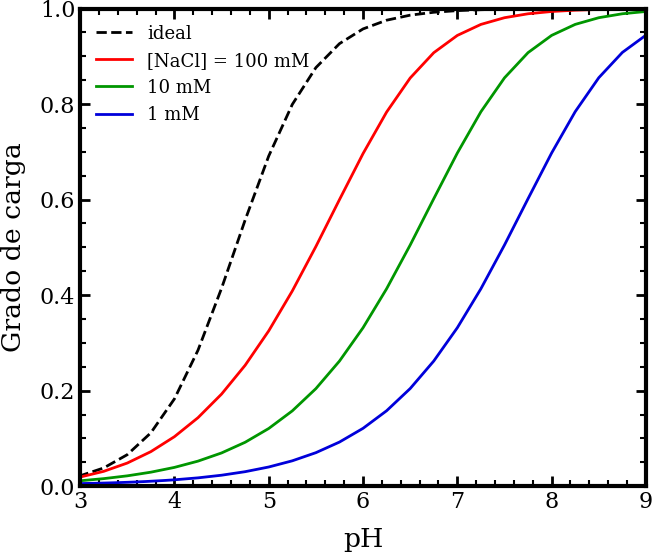
\includegraphics[width=0.9\textwidth]{Figures/graph-film/charge_degree-film.png}
    \caption{Grado de carga del gel como funci\'on del pH. Grado de carga para un monomero aislado en presentado en curva a rayas, se compara para diferentes concentraciones de sal, a mayor concentraci\'on salina m\'as nos acercamos al sistema ideal.}
    \label{fig:film:degree-film}
\end{figure}

A un pH dado, es significativamente menos probable que una unidad \'acida de la red polim\'erica se cargue en comparaci\'on con las consideraciones ideales. La concentraci\'on de sal en la soluci\'on resulta ser una variable cr\'itica que modula este comportamiento de regulaci\'on de carga.

A una salinidad relativamente alta, la cantidad de contraiones dentro del film aumenta, lo que resulta en el apantallamiento de las interacciones electrost\'aticas. Estas interacciones se vuelven de corto alcance. Este apantallamiento de repulsiones dentro de la red permite que el pol\'imero aumente su grado de carga. En esta observaci\'on inicial, vemos que un aumento en la salinidad genera una protonaci\'on que se aproxima al comportamiento ideal.

En condiciones de baja concentraci\'on de sal, solo hay suficientes contraiones dentro de la red para neutralizar la carga el\'ectrica del pol\'imero. Bajo estas condiciones, el efecto de apantallamiento de los iones de sal se debilita y las interacciones electrost\'aticas efectivamente tienen un mayor alcance. Como resultado, la red se carga menos para prevenir o reducir las repulsiones dentro de la red.

En la figura \ref{fig:film:degree-film}, se observa que el grado de carga de los films polim\'ericos difiere del comportamiento de los mon\'omeros aislados. Esto nos lleva a pensar que las condiciones en este entorno son diferentes a las que se esperar\'ian en la soluci\'on. Existe una regulaci\'on de carga, lo que sugiere una regulaci\'on del pH.

Definimos as\'i el pH local, que nos proporciona la concentración de protones en una posición espacial $z$

\begin{equation}
	pH(z) = -\log_{10}(H^+)
	\label{eq:film:pH-local}
\end{equation}

Una baja disociaci\'on (un alto nivel de protonaci\'on) de las unidades \'acidas de las unidades de MAA en nuestra red polim\'erica puede explicarse en t\'erminos del pH local dentro del material. Definimos el pH del gel ($pH_{gel}$) como el promedio del pH local dentro del film. Resultados previos han mostrado que esta cantidad est\'a bien definida \cite{longo2014non}.

Enfatizamos la importancia de estos dos t\'erminos, $pH_{gel}$ y $pH(z)$, por la informaci\'on que proporcionan: el estado de carga/protonaci\'on de las unidades titulables en la red polim\'erica.

Haciendo uso de la ecuaci\'on \ref{eq:film:diso-ideal}, es posible calcular el grado de disociaci\'on de la estructura polim\'erica de nuestro hidrogel. El uso de $pH_{gel}$ es indispensable en condiciones en las que el pH difiere del pH de la soluci\'on . El mismo procedimiento se realiza para calcular el estado de protonaci\'on local de las unidades titulables de las especies que se adsorben en el film (ver figura \ref{fig:film:protein-charge}).


\begin{figure}
    \centering
    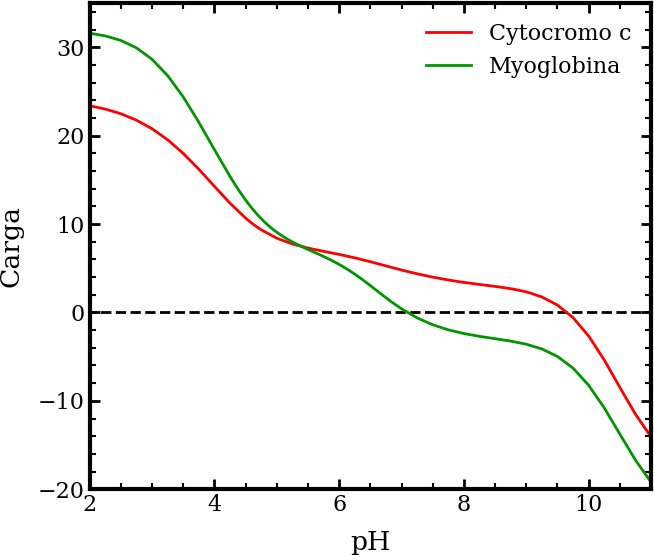
\includegraphics[width=0.9\textwidth]{Figures/graph-film/carga-proteinas.png}
    \caption{N\'umero de carga de las proteinas cytocromo c y myoglobina como  funci\'on del pH en el seno de la soluci\'on (bulk). La l\'inea a trazos muestra el cambio en el signo de la carga.}
    \label{fig:film:protein-charge}
\end{figure}


Sin embargo, aunque esto parece simplificar el problema de establecer la carga neta de cualquier especie del sistema, en nuestro caso la red polim\'erica y las prote\'inas adsorbidas, determinar los cambios en el pH local tiene la misma complejidad que el problema original (es decir, la de determinar la carga del film). El pH local que se establece dentro del material, as\'i como su valor en la interfaz entre el film polim\'erico y la soluci\'on acuosa, es el resultado de la compleja interacci\'on entre la organizaci\'on molecular, los equilibrios qu\'imicos y las interacciones f\'isicas que determinan el equilibrio termodin\'amico en las condiciones impuestas externamente (pH, concentraci\'on de sal). Todas las variables expuestas se describen en la secci\'on \ref{sec:film-teoria}.

Para ejemplificar c\'omo varí\'i el pH en relaci\'on con el pH y la concentraci\'on salina dada en el bulk de la soluci\'on, se puede observar la figura \ref{fig:film:pH-local}, que muestra el pH dentro de nuestro film de cadenas de 
PMAA
PMAA como funci\'on del pH. Cada curva hace referencia a una concentraci\'on de sal diferente. Se agrega, a rayas, el comportamiento ``ideal" en el que el pH del bulk es igual al pH local, en particular al del film, calculado usando teor\'ia molecular.


\begin{figure}
    \centering
    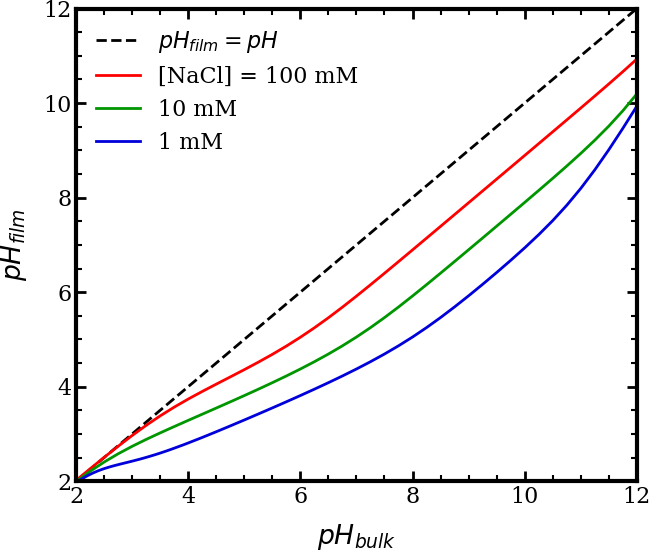
\includegraphics[width=0.9\textwidth]{Figures/graph-film/pH-local.png}
    \caption{pH local del gel como funci\'on del pH en el seno de la soluci\'on (bulk). Cada curva corresponde a una concentraci\'on de sal diferente.}
    \label{fig:film:pH-local}
\end{figure}

\subsection{Adsorci\'on}\label{sec:film:resu-absorcion}

El uso estos sistemas de hidrogeles como transportadores de adsrobatos de utilidad terap\'eutica, involucra el poder cuantificar y cualificar esta adsorci\'on.
 
Para ello nos valdremos de la teor\'ia molecular ya expuesta y haciendlo uso de ciertas prote\'inas modelo como lo son el citocromo c y la mioglobina. El uso de estas dos porte\'inas presentan gran estabilidad en un amplio rango de pH, y contar con estudios experimentales en sistemas polim\'ericos similares.

El uso de hidrogeles como transportadores de adsorbatos con fines terap\'euticos ha despertado un gran inter\'es en la comunidad cient\'ifica. Sin embargo, para aprovechar al m\'aximo su potencial, es fundamental poder cuantificar y cualificar la adsorci\'on de mol\'eculas y prote\'inas en estos sistemas.

En este sentido, recurrimos a la teor\'ia molecular previamente expuesta, la cual nos brinda herramientas para comprender y predecir la interacci\'on entre las prote\'inas y el hidrogel polim\'erico. Para estos  modelos te\'oricos, seleccionamos prote\'inas modelo con estabilidad en un amplio rango de pH, como el citocromo c y la mioglobina. Estas prote\'inas han sido ampliamente estudiadas en sistemas polim\'ericos similares, lo que nos permite aprovechar la experiencia acumulada de estas investigaciones previas.

Para cuantificar la cantidad de prote\'ina adsorbida en el film de hidrogel, empleamos la siguiente  expresi\'on:

\begin{align}
\Gamma_{pro} = \int^\infty_0 {dz(\rho_{pro}(z) -\rho^b_{pro}}  
\label{eq:film:adsor-exceso}
\end{align}


En donde $\rho_{\text{pro}}(z)$ y $\rho^b_{\text{pro}}$ son las densidades locales y en el bulk de la soluci\'on de la prote\'ina, respectivamente.
$\Gamma_{\text{pro}}$ proporciona la cantidad de adsorbato por unidad de \'area en exceso dentro del material, recibiendo tambi\'en contribuciones de la interfaz de soluci\'on de pol\'imero.

Para estas prote\'inas, la adsorci\'on es una funci
'on no mon\'otona del pH de la soluci\'on (ver Figura \ref{fig:film:ad-pro}). A pH bajo, estas prote\'inas tienen una carga alta y positiva, pero la red de poli\'acidos ($PMAA$) solo est\'a d\'ebilmente ionizada (v\'eanse las Figuras \ref{fig:film:degree-film} y \ref{fig:film:protein-charge}). A un pH suficientemente alto, por otro lado, el pol\'imero est\'a fuertemente cargado negativamente, pero las prote\'inas tienen una carga d\'ebilmente positiva o incluso negativa. Bajo tales condiciones (muy) \'acidas o alcalinas, las interacciones electrost\'aticas son d\'ebilmente atractivas o repulsivas, respectivamente. No hay fuerza impulsora para la adsorci\'on. A valores de pH intermedios, por el contrario, donde tanto la prote\'ina como la red polim\'erica tienen cargas fuertes y opuestas, se produce una adsorci\'on significativa con un m\'aximo necesario en tales condiciones.

La adsorci\'on de prote\'inas depende cr\'iticamente de la concentraci\'on de sal de la soluci\'on. Este comportamiento se ilustra en la figura \ref{fig:film:ad-pro}, que muestra la adsorci\'on de citocromo c y mioglobina en un film compuesto por cadenas polim\'ericas de $PMAA$. La disminuci\'on de las concentraciones de sal mejora la adsorci\'on y ampl\'ia el rango de pH de la adsorci\'on.
Por ejemplo, ambos paneles de la figura \ref{fig:film:ad-pro} muestran una disminuci\'on de aproximadamente un orden de magnitud en la adsorci\'on cuando se comparan soluciones de NaCl 1 mM y 10 mM.
El pH de m\'axima adsorci\'on tambi\'en depende de la salinidad de la soluci\'on. Este comportamiento es a\'un m\'as interesante cuando se considera que una concentraci\'on de sal m\'as baja conduce a una red con carga m\'as d\'ebil, como describimos anteriormente, fig. \ref{fig:film:degree-film}.
En otras palabras, a medida que disminuye la concentraci\'on de sal, m\'as prote\'ina es adsorbida. Esta \'ultima afirmaci\'on es cierta en las concentraciones de prote\'ina ($10 \mu M$) y sal de la figura \ref{fig:film:ad-pro}, donde la adsorci\'on solo modifica ligeramente el grado de carga de la red.

Esta dependencia de la adsorci\'on de la concentraci\'on de sal tiene tres razones principales: en primer lugar, existe el apantallamiento de las atracciones electrost\'aticas de la red hacia las prote\'inas por parte de los iones de sal.
Cuanto menor sea la concentraci\'on de sal, m\'as d\'ebil ser\'a el apantallamiento de las interacciones prote\'ina-red, lo que mejora la adsorci\'on.




\begin{figure}
    \centering
    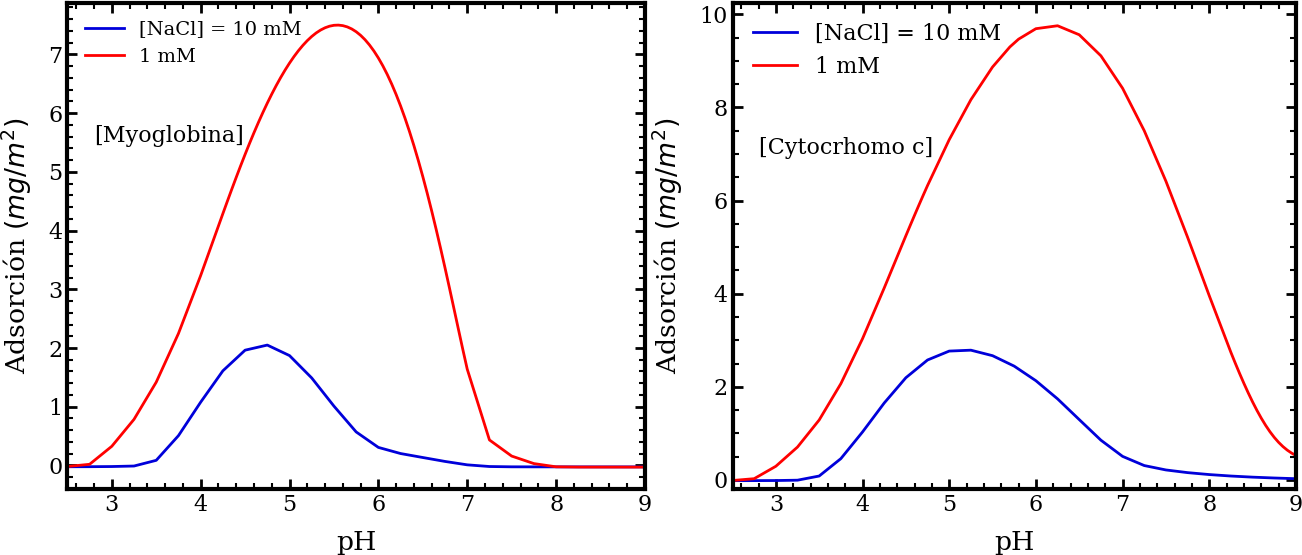
\includegraphics[width=0.99\textwidth]{Figures/graph-film/ad-proteins.png}
    \caption{Adsorci\'on de proteinas: cytocromo c y myoglobina en panel A y B respectivamente. La concentraci\'on de los adsorbatos es $10 \mu M$}
    \label{fig:film:ad-pro}
\end{figure}


\section{Conclusiones}


Los hidrogeles de polim\'ericos sensibles al pH son prometedores candidatos para biomateriales inteligentes y responsivos, lo cual impone la necesidad de comprender su compleja interacción fisicoqu\'imica con las prote\'inas. Las simulaciones moleculares pueden proporcionar informaci\'on perspicaz para comprender los mecanismos detr\'as de la adsorci\'on de prote\'inas en geles sensibles al pH, lo cual puede ser dif\'icil o imposible de obtener mediante experimentos. En este cap\'itulo se ha tratado de  entender y explicar el estado de protonaci\'on de la red polim\'erica de los filmes de hidrogel y el de los diferentes residuos de amino\'acidos de las prote\'inas afectan o modulan su interacci\'on. Hemos demostrado que un comportamiento rico emerge de la capacidad de la prote\'ina para regular su carga el\'ectrica en el entorno de pH m\'as bajo que ocurre dentro del material. Este comportamiento se puede utilizar para la separaci\'on o localizaci\'on de prote\'inas dentro de regiones espaciales de tama\~no nanom\'etrico dentro del material. Imaginamos, por ejemplo, el desarrollo de materiales multifuncionales basados en hidrogel donde diferentes proteínas son activas en diferentes regiones de la red polim\'erica. Exploraremos te\'oricamente estos conceptos en los pr\'oximos cap\'itulos cuando los traslados a los microgeles y nanogles cap\'itulos  \ref{Chapter-geles}  y \ref{Chapter-esfericas} respectivamente.
